\documentclass[english, aspectratio=169]{beamer}
% english is for the language used in standard texts (figures, tables etc)
% aspectratio of 16:9 or set it for more old school to 4:3 (without the ':')

% ---------------------------------------------------------------------------- %
% Load base preamble
% ---------------------------------------------------------------------------- %
\usepackage{import}
\subimport{./preamble/}{beamer.tex}

\metroset{sectionpage=none}

% ---------------------------------------------------------------------------- %
% Local settings
% ---------------------------------------------------------------------------- %
\lstset{
  language = none,
  basicstyle=\footnotesize\ttfamily
}

\usepackage{ragged2e}

% https://tex.stackexchange.com/a/460764
\usepackage{soul}
\makeatletter
\let\HL\hl
\renewcommand\hl{%
  \let\set@color\beamerorig@set@color
  \let\reset@color\beamerorig@reset@color
  \HL}
\makeatother

% https://tex.stackexchange.com/a/20613
\newcommand\hcancel[2][black]{\setbox0=\hbox{$#2$}%
  \rlap{\raisebox{.35\ht0}{\textcolor{#1}{\rule{\wd0}{1pt}}}}#2}

\newcommand{\B}[0]{\ensuremath{\mathbb{B}}}
\newcommand{\ns}[0]{\ensuremath{\mathit{ns}}}
\newcommand{\pq}[0]{\ensuremath{\texttt{pq}}}
\newcommand{\vc}[0]{\ensuremath{\texttt{vc}}}

\newcommand{\countReq}[0]{\ensuremath{\#^{\texttt{Req}}}}
\newcommand{\countPQ}[0]{\ensuremath{\#^{\pq}}}

\newcommand{\sort}[0]{\text{sort}}

\newcommand{\triple}[3]{\ensuremath{(#1, #2, #3)}}
\renewcommand{\arc}[3]{\ensuremath{#1 \xrightarrow{_{#2}} #3}}

% Horizontal legends: https://tex.stackexchange.com/a/101578
% argument #1: any options
\makeatletter
\newenvironment{customlegend}[1][]{%
    \begingroup
    % inits/clears the lists (which might be populated from previous
    % axes):
    \pgfplots@init@cleared@structures
    \pgfplotsset{#1}%
}{%
    % draws the legend:
    \pgfplots@createlegend
    \endgroup
}%

% makes \addlegendimage available (typically only available within an
% axis environment):
\def\addlegendimage{\pgfplots@addlegendimage}
\makeatother

% ------------------------------------------------------------------------------------------------ %
% TITLEPAGE
% ------------------------------------------------------------------------------------------------ %
\title{Correctness of Time-forward Processing Algorithms}

\author{{\bf Steffan S{\o}lvsten}, Simon Wimmer}

\institute{
\includegraphics[width=0.2\linewidth]{external/aulogo_uk_var2_black.eps}}

\date{LogSem Seminar, 2\textsuperscript{nd} of December 2024}

\begin{document}

\titleframe

% ------------------------------------------------------------------------------------------------ %
% MOTIVATION
% ------------------------------------------------------------------------------------------------ %
\section{Motivation}

\begin{frame}[plain,noframenumbering]
  \begin{center}
    {\fontsize{42}{50}\selectfont \textbf{Adiar}}

    \textcolor{gray}{\large \em
      I/O-efficient Decision Diagrams
    }

    \vspace{-10pt}
    \rule{180pt}{0.6pt}
    \vspace{-5pt}

    \textcolor{gray}{\small
      \href{http://github.com/logsem/adiar}{github.com/logsem/adiar}
    }
  \end{center}
\end{frame}

\begin{frame}[plain,noframenumbering]
  \begin{figure}
    \centering

    \tikzstyle{plot_adiar} =[color=red,    mark=diamond*,  mark size=1pt, line width=0.7pt, mark options={color=red,    fill=red}]
    \tikzstyle{plot_buddy} =[color=purple, mark=pentagon*, mark size=1pt, line width=0.7pt, mark options={color=purple, fill=purple}]
    \tikzstyle{plot_cudd}  =[color=orange, mark=triangle*, mark size=1pt, line width=0.7pt, mark options={color=orange, fill=orange}]
    \tikzstyle{plot_sylvan}=[color=cyan,   mark=*,         mark size=1pt, line width=0.7pt, mark options={color=cyan,   fill=cyan}]

    \begin{tikzpicture}
      \begin{axis}[%
        width=0.88\linewidth, height=0.42\linewidth,
        every tick label/.append style={font=\scriptsize},
        % x-axis
        xlabel={Problem Complexity (\# BDD nodes)},
        xmajorgrids=true,
        xmin=12000,
        xmax=300000000000,
        xmode = log,
        % y-axis
        ymin=0.001,
        ymax=1000000,
        ymode=log,
        ytick={0.001,0.01,0.1,1,10,100,1000,10000,100000,1000000},
        ylabel={Time (s)},
        yminorgrids=false,
        ymajorgrids=true,
        grid style={dashed,black!20},
        ]

        \addplot+ [style=plot_buddy]
        table {./data/queens_buddy_time.tex};

        \addplot+ [style=plot_cudd]
        table {./data/queens_cudd_time.tex};

        \addplot+ [style=plot_sylvan]
        table {./data/queens_sylvan_time.tex};

        \addplot+ [style=plot_adiar]
        table {./data/queens_adiar_time.v1.2.0.tex};
      \end{axis}
    \end{tikzpicture}

    \begin{tikzpicture}
      \begin{customlegend}[
        legend columns=-1,
        legend style={draw=none,column sep=1ex},
        legend entries={Adiar, BuDDy, CUDD, Sylvan}
        ]
        \addlegendimage{style=plot_adiar}
        \addlegendimage{style=plot_buddy}
        \addlegendimage{style=plot_cudd}
        \addlegendimage{style=plot_sylvan}
      \end{customlegend}
    \end{tikzpicture}

    \caption{Running Time to solve $N$-\emph{Queens} problems.}
  \end{figure}
\end{frame}

\begin{frame}[plain,noframenumbering]
  \begin{figure}
    \centering

    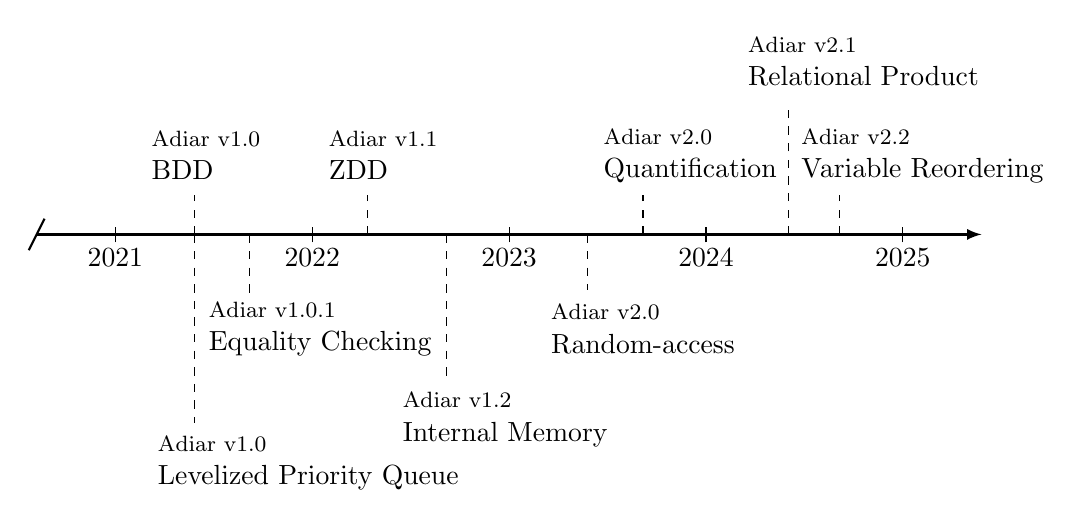
\begin{tikzpicture}
      % Primary line
\draw[-latex, thick] (0,0) -- (12,0);
\draw[thick] (0.1,0.2) -- (-0.1,-0.2);

% 2021
\draw (1,-0.1) -- ++(0,0.2);
\node at (1,-0.3) {$2021$};

\draw[dashed, color=black] (2,0) -- ++(0,0.5);
\node[color=black, align=left] at (2.15,1.0)
{\footnotesize Adiar v1.0\\BDD};

\draw[dashed, color=black] (2,0) -- ++(0,-2.4);
\node[color=black, align=left] at (3.45,-2.9)
{\footnotesize Adiar v1.0\\Levelized Priority Queue};

\draw[dashed, color=black] (2.7,0) -- ++(0,-0.8);
\node[color=black, align=left] at (3.6,-1.2)
{\footnotesize Adiar v1.0.1\\Equality Checking};

% 2022
\draw (3.5,-0.1) -- ++(0,0.2);
\node at (3.5,-0.3) {$2022$};

\draw[dashed, color=black] (4.2,0) -- ++(0,0.5);
\node[color=black, align=left] at (4.4,1.0)
{\footnotesize Adiar v1.1\\ZDD};

\draw[dashed, color=black] (5.2,0) -- ++(0,-1.8);
\node[color=black, align=left] at (5.95,-2.35)
{\footnotesize Adiar v1.2\\Internal Memory};

% 2023
\draw (6,-0.1) -- ++(0,0.2);
\node at (6,-0.3) {$2023$};

\draw[dashed, color=black] (7,0) -- ++(0,-0.7);
\node[color=black, align=left] at (7.7,-1.2)
{\footnotesize Adiar v2.0\\Random-access};

\draw[dashed, color=black] (7.7,0) -- ++(0,0.5);
\node[color=black, align=left] at (8.3,1.0)
{\footnotesize Adiar v2.0\\Quantification};

% 2024
\draw (8.5,-0.1) -- ++(0,0.2);
\node at (8.5,-0.3) (y2024) {$2024$};

\draw[dashed, color=black] (9.55,0) -- ++(0,1.6);
\node[color=black, align=left] at (10.5,2.2)
{\footnotesize Adiar v2.1\\Relational Product};

\draw[dashed, color=black] (10.2,0) -- ++(0,0.5);
\node[color=black, align=left] at (11.25,1.0)
{\footnotesize Adiar v2.2\\Variable Reordering};

% 2025
\draw (11,-0.1) -- ++(0,0.2);
\node at (11,-0.3) (y2025) {$2025$};
    \end{tikzpicture}
  \end{figure}
\end{frame}

\begin{frame}[plain,noframenumbering]
  \begin{center}
    {\LARGE Written in}

    \medskip

    {\fontsize{42}{50}\selectfont \textbf{C++}}
  \end{center}
\end{frame}

\begin{frame}[plain, noframenumbering, fragile]
  \begin{lstlisting}[numbers=none]
  //////////////////////////////////////////////////////////////////
  /// \brief Negates the content of `p` if it is a terminal and the
  ///        `negate` flag is set to true.
  //////////////////////////////////////////////////////////////////
  \end{lstlisting}
  \begin{lstlisting}
  inline ptr_uint64
  cnot(const ptr_uint64& p, const bool negate)
  {
    const uint64 shifted_negate =
      ((uint64) negate) << ptr_uint64::data_shift;
    return p.is_leaf() ? p._raw ^ shifted_negate : p._raw;
  }
  \end{lstlisting}
\end{frame}

\begin{frame}[plain,noframenumbering]
  \begin{center}
    {\LARGE Correctness guaranteed by}

    {\Huge
      \textbf{$\sim$3500 Unit Tests}

      \bigskip

      \textbf{$\sim$400 Integration Tests}
    }
  \end{center}
\end{frame}

\blankframe

\begin{frame}[plain,noframenumbering]
  \begin{center}
    {\Large\bf Cache and I/O Efficient Functional Algorithms}

    Guy E. Blelloch \qquad Robert Harper

    {\footnotesize Carnegie Mellon University}
  \end{center}

  \begin{block}{Abstract}
    \justifying \fontsize{8}{9}\selectfont

    In this paper we present a cost model for analyzing the memory efficiency of algorithms
    expressed in a simple functional language. We show how some algorithms written in standard forms
    using just lists and trees (no arrays) and requiring no explicit memory layout or memory
    management are efficient in the model. We then describe an implementation of the language and
    show provable bounds for mapping the cost in our model to the cost in the ideal- cache model.
    \hl{These bound imply that purely functional programs based on lists
      and trees with no special attention to any details of memory layout can be as asymptotically
      as efficient as the carefully designed imperative I/O efficient algorithms.} For example we
    describe an $\Oh{N/B \log_{M/B} N/B}$ cost sorting algorithm, which is optimal in the ideal
    cache and I/O models.
  \end{block}
\end{frame}

\blankframe

% ------------------------------------------------------------------------------------------------ %
\section{Correctness of Time-forward Processing}

\begin{frame}[plain,noframenumbering]{}
  \frametitle{Contents}
  \tableofcontents
\end{frame}

% ------------------------------------------------------------------------------------------------ %
% BDD + DATA TYPES
% ------------------------------------------------------------------------------------------------ %
\subsection{Encoding Binary Decision Diagrams}

\begin{frame}[plain,noframenumbering]{}
  \frametitle{Contents}
  \tableofcontents[currentsection,currentsubsection]
\end{frame}

\begin{frame}
  \frametitle{Semantics of BDDs}

  \only<1>{
    \begin{center}
      \huge

      $f(x_0, x_1, x_2, x_3) \equiv (x_0 \wedge x_1 \wedge x_3) \vee (x_2 \oplus x_3)$
    \end{center}
  }
  \only<2>{
    \begin{figure}
      \begin{tikzpicture}[scale=0.9, every node/.style={transform shape}]
        % nodes
        \node[shape = circle, draw = black]
        (0) {$x_0$};

        \node[shape = circle, draw = black, below left=.4cm and 3.0cm of 0]
        (1a) {$x_1$};
        \node[shape = circle, draw = black, below right=.4cm and 3.0cm of 0]
        (1b) {$x_1$};

        \node[shape = circle, draw = black, below left=0.4cm and 1.2cm of 1a]
        (2a) {$x_2$};
        \node[shape = circle, draw = black, below right=0.4cm and 1.2cm of 1a]
        (2b) {$x_2$};
        \node[shape = circle, draw = black, below left=0.4cm and 1.2cm of 1b]
        (2c) {$x_2$};
        \node[shape = circle, draw = black, below right=0.4cm and 1.2cm of 1b]
        (2d) {$x_2$};

        \node[shape = circle, draw = black, below left=.4cm and .3cm of 2a]
        (3a) {$x_3$};
        \node[shape = circle, draw = black, below right=.4cm and .3cm of 2a]
        (3b) {$x_3$};
        \node[shape = circle, draw = black, below left=.4cm and .3cm of 2b]
        (3c) {$x_3$};
        \node[shape = circle, draw = black, below right=.4cm and .3cm of 2b]
        (3d) {$x_3$};
        \node[shape = circle, draw = black, below left=.4cm and .3cm of 2c]
        (3e) {$x_3$};
        \node[shape = circle, draw = black, below right=.4cm and .3cm of 2c]
        (3f) {$x_3$};
        \node[shape = circle, draw = black, below left=.4cm and .3cm of 2d]
        (3g) {$x_3$};
        \node[shape = circle, draw = black, below right=.4cm and .3cm of 2d]
        (3h) {$x_3$};

        % leafs
        \node[shape = rectangle, draw = black, below left=.4cm and -0.1cm of 3a]
        (Sa) {$\top$};
        \node[shape = rectangle, draw = black, below right=.4cm and -0.1cm of 3a]
        (Sb) {$\bot$};
        \node[shape = rectangle, draw = black, below left=.4cm and -0.1cm of 3b]
        (Sc) {$\bot$};
        \node[shape = rectangle, draw = black, below right=.4cm and -0.1cm of 3b]
        (Sd) {$\top$};
        \node[shape = rectangle, draw = black, below left=.4cm and -0.1cm of 3c]
        (Se) {$\top$};
        \node[shape = rectangle, draw = black, below right=.4cm and -0.1cm of 3c]
        (Sf) {$\bot$};
        \node[shape = rectangle, draw = black, below left=.4cm and -0.1cm of 3d]
        (Sg) {$\bot$};
        \node[shape = rectangle, draw = black, below right=.4cm and -0.1cm of 3d]
        (Sh) {$\top$};
        \node[shape = rectangle, draw = black, below left=.4cm and -0.1cm of 3e]
        (Si) {$\top$};
        \node[shape = rectangle, draw = black, below right=.4cm and -0.1cm of 3e]
        (Sj) {$\bot$};
        \node[shape = rectangle, draw = black, below left=.4cm and -0.1cm of 3f]
        (Sk) {$\bot$};
        \node[shape = rectangle, draw = black, below right=.4cm and -0.1cm of 3f]
        (Sl) {$\top$};
        \node[shape = rectangle, draw = black, below left=.4cm and -0.1cm of 3g]
        (Sm) {$\bot$};
        \node[shape = rectangle, draw = black, below right=.4cm and -0.1cm of 3g]
        (Sn) {$\top$};
        \node[shape = rectangle, draw = black, below left=.4cm and -0.1cm of 3h]
        (So) {$\bot$};
        \node[shape = rectangle, draw = black, below right=.4cm and -0.1cm of 3h]
        (Sp) {$\top$};

        % arcs
        \draw[->, dashed]
        (0)  edge (1a)
        (1a) edge (2a)
        (1b) edge (2c)
        (2a) edge (3a)
        (2b) edge (3c)
        (2c) edge (3e)
        (2d) edge (3g)
        (3a) edge (Sa)
        (3b) edge (Sc)
        (3c) edge (Se)
        (3d) edge (Sg)
        (3e) edge (Si)
        (3f) edge (Sk)
        (3g) edge (Sm)
        (3h) edge (So)
        ;

        \draw[->]
        (0)  edge (1b)
        (1a) edge (2b)
        (1b) edge (2d)
        (2a) edge (3b)
        (2b) edge (3d)
        (2c) edge (3f)
        (2d) edge (3h)
        (3a) edge (Sb)
        (3b) edge (Sd)
        (3c) edge (Sf)
        (3d) edge (Sh)
        (3e) edge (Sj)
        (3f) edge (Sl)
        (3g) edge (Sn)
        (3h) edge (Sp)
        ;
      \end{tikzpicture}

      \caption{Binary Decision Tree}
    \end{figure}
  }
  \only<3>{
    \begin{figure}
      \centering

      \begin{tikzpicture}[scale=0.875, every node/.style={transform shape}]
          % nodes
  \node[shape = circle, draw = black]
  (0) {$x_0$};

  \node[shape = circle, draw = black, below right= .4cm and .5cm of 0]
  (1) {$x_1$};

  \node[shape = circle, draw = black, below left=.4cm and .5cm of 1]
  (2) {$x_2$};

  \node[shape = circle, draw = black, below left=.4cm and .5cm of 2]
  (31) {$x_3$};
  \node[shape = circle, draw = black, below right=.4cm and .5cm of 2]
  (32) {$x_3$};

  % leafs
  \node[shape = rectangle, draw = black, below=.4cm of 31]
  (sink_T) {$\top$};

  \node[shape = rectangle, draw = black, below=.4cm of 32]
  (sink_F) {$\bot$};

  % arcs
  \draw[->, dashed]
    (0)  edge (2)
    (1)  edge (2)
    (2)  edge (31)
    (31) edge (sink_T)
    (32) edge (sink_F)
  ;

  \draw[->]
    (0)  edge (1)
    (1)  edge (32)
    (2)  edge (32)
    (31) edge (sink_F)
    (32) edge (sink_T)
  ;
      \end{tikzpicture}

      \caption{Binary Decision Diagram}
    \end{figure}
  }

  \footnotetext[1]{Julius Michaelis, Maximilian Haslbeck, Peter Lammich, and Lars Hupel. “Algorithms
    for Reduced Ordered Binary Decision Diagrams”. In: Archive of Formal Proofs (2016)}
\end{frame}

\begin{frame}[fragile]
  \frametitle{Data Types: Unique Identifiers and Pointers}

  \begin{lstlisting}
Uid = (level: $\N$, id: $\N$)
  \end{lstlisting}
  \begin{lstlisting}[firstnumber=2]
operator < (a: Uid) (b: Uid) =
    a.level < b.level $\lor$ (a.level = b.level $\land$ a.id < b.id)
  \end{lstlisting}

  \begin{lstlisting}[firstnumber=4]
Ptr = Leaf (val : $\B$)
    | Node (uid : Uid)
  \end{lstlisting}
  \begin{lstlisting}[firstnumber=5]
operator < (a: Ptr) (b: Ptr) =
    lift Uid.< s.t. Ptr.Node < Ptr.Leaf
  \end{lstlisting}

  \begin{lemma}
    \texttt{Uid}.$<$ and \texttt{Ptr}.$<$ are total orders.
  \end{lemma}
  \begin{proof}
    Trival case distinctions.
  \end{proof}
\end{frame}

\begin{frame}[t, fragile]
  \frametitle{Data Types: Nodes and BDDs}

  \begin{columns}
    \begin{column}[t]{0.4\linewidth}
      \begin{figure}
        \centering

        \begin{tikzpicture}[every node/.style={transform shape}]
            % nodes
  \node[shape = circle, draw = black]
  (0) {$x_0$};

  \node[shape = circle, draw = black, below right= .4cm and .5cm of 0]
  (1) {$x_1$};

  \node[shape = circle, draw = black, below left=.4cm and .5cm of 1]
  (2) {$x_2$};

  \node[shape = circle, draw = black, below left=.4cm and .5cm of 2]
  (31) {$x_3$};
  \node[shape = circle, draw = black, below right=.4cm and .5cm of 2]
  (32) {$x_3$};

  % leafs
  \node[shape = rectangle, draw = black, below=.4cm of 31]
  (sink_T) {$\top$};

  \node[shape = rectangle, draw = black, below=.4cm of 32]
  (sink_F) {$\bot$};

  % arcs
  \draw[->, dashed]
    (0)  edge (2)
    (1)  edge (2)
    (2)  edge (31)
    (31) edge (sink_T)
    (32) edge (sink_F)
  ;

  \draw[->]
    (0)  edge (1)
    (1)  edge (32)
    (2)  edge (32)
    (31) edge (sink_F)
    (32) edge (sink_T)
  ;
        \end{tikzpicture}

        \caption{$(x_0 \wedge x_1 \wedge x_3) \vee (x_2 \oplus x_3)$}
      \end{figure}
    \end{column}
    \begin{column}[t]{0.6\linewidth}
      \begin{lstlisting}
Node = (i: Uid, t: Ptr, e: Ptr)
Bdd  = Leaf  (val : $\B$)
     | Nodes (ns : List[Node])
      \end{lstlisting}

      \begin{lstlisting}[firstnumber=4]
Example = Bdd.Nodes([
  Node(Uid(0,0), Ptr(1,0), Ptr(2,0));
  Node(Uid(1,0), Ptr(3,1), Ptr(2,0));
  Node(Uid(2,0), Ptr(3,1), Ptr(3,0));
  Node(Uid(3,0), Ptr($\bot$),    Ptr($\top$));
  Node(Uid(3,1), Ptr($\top$),    Ptr($\bot$));
])
      \end{lstlisting}
    \end{column}
  \end{columns}
\end{frame}

\begin{frame}[t, fragile, noframenumbering] % hack to not increment slide counter
  \frametitle{Data Types: Nodes and BDDs}

  \begin{columns}
    \begin{column}[t]{0.4\linewidth}
      \begin{figure}
        \centering

        \begin{tikzpicture}[every node/.style={transform shape}]
            % nodes
  \node[shape = circle, draw = black]
  (0) {$x_0$};

  \node[shape = circle, draw = black, below right= .4cm and .5cm of 0]
  (1) {$x_1$};

  \node[shape = circle, draw = black, below left=.4cm and .5cm of 1]
  (2) {$x_2$};

  \node[shape = circle, draw = black, below left=.4cm and .5cm of 2]
  (31) {$x_3$};
  \node[shape = circle, draw = black, below right=.4cm and .5cm of 2]
  (32) {$x_3$};

  % leafs
  \node[shape = rectangle, draw = black, below=.4cm of 31]
  (sink_T) {$\top$};

  \node[shape = rectangle, draw = black, below=.4cm of 32]
  (sink_F) {$\bot$};

  % arcs
  \draw[->, dashed]
    (0)  edge (2)
    (1)  edge (2)
    (2)  edge (31)
    (31) edge (sink_T)
    (32) edge (sink_F)
  ;

  \draw[->]
    (0)  edge (1)
    (1)  edge (32)
    (2)  edge (32)
    (31) edge (sink_F)
    (32) edge (sink_T)
  ;
        \end{tikzpicture}

        \caption{$(x_0 \wedge x_1 \wedge x_3) \vee (x_2 \oplus x_3)$}
      \end{figure}
    \end{column}
    \begin{column}[t]{0.6\linewidth}
      \begin{lstlisting}
Node = (i: Uid, t: Ptr, e: Ptr)
Bdd  = Leaf  (val : $\B$)
     | Nodes (ns : List[Node])
      \end{lstlisting}

      \begin{definition}
        A \texttt{Bdd} is \emph{well formed}, if \texttt{ns}~:~\texttt{List[Node]} satisfies:
        \begin{enumerate}
        \item It is \emph{non-empty}.
        \item It is \emph{closed}, i.e.\ every node referred to exists.
        \item For each node, the level is strictly increasing.
        \item It is \emph{sorted} w.r.t.\ \texttt{Node.i}.
        \end{enumerate}
      \end{definition}
    \end{column}
  \end{columns}
\end{frame}

% ------------------------------------------------------------------------------------------------ %
% BDD EVAL
% ------------------------------------------------------------------------------------------------ %
\subsection{bbd\_eval}

\begin{frame}[plain,noframenumbering]{}
  \frametitle{Contents}
  \tableofcontents[currentsection,currentsubsection]
\end{frame}

\begin{frame}[fragile]
  \frametitle{bdd\_eval f x}

  \begin{lstlisting}
bdd_eval' ((i t e)::ns': List[Node]) (tgt: Uid) (x: $\N \rightarrow \B$) =
    if i < tgt
    then bdd_eval' ns' tgt x
    else match (x(a) ? t : e) with
             | Leaf(b)    => b
             | Node(tgt') => bdd_eval' ns' tgt' x
   \end{lstlisting}
   \begin{lstlisting}[firstnumber=7]
bdd_eval (val   : Bdd.Leaf)  (x: $\N \rightarrow \B$) = val
bdd_eval (r::ns : Bdd.Nodes) (x: $\N \rightarrow \B$) = bdd_eval' r::ns r x
  \end{lstlisting}
\end{frame}

\begin{frame}
  \frametitle{bdd\_eval f x}

  Define the function \texttt{bdt\_of\_bdd}~:~$\texttt{Bdd} \rightarrow \texttt{Bdt}$ to converts a
  Binary Decision Diagram into a Binary Decision Tree. Here, skip over ``irrelevant'' nodes to
  convert subtrees.

  \pause

  \begin{theorem}
    If $f$ is \emph{well formed}, then $\forall x$:
    $\texttt{bdd\_eval f x} \iff \texttt{bdt\_eval (bdt\_of\_bdd f) x}$.
  \end{theorem}
  \begin{proof}
    Case \texttt{Leaf} $\B$: Trivial

    Case \texttt{Nodes ns}:\\
    \quad Induction on \texttt{ns}.\\
    \quad Discard bad cases due to the BDD being \emph{closed} and \emph{sorted}.
  \end{proof}
\end{frame}

% ------------------------------------------------------------------------------------------------ %
% BDD NOT
% ------------------------------------------------------------------------------------------------ %
\subsection{bbd\_not}

\begin{frame}[plain,noframenumbering]{}
  \frametitle{Contents}
  \tableofcontents[currentsection,currentsubsection]
\end{frame}

\begin{frame}[fragile]
  \frametitle{bdd\_not f}

  \begin{lstlisting}
operator ! (p: Ptr) = match p with
                          | Leaf v => !v
                          | Node u => u
  \end{lstlisting}
  \begin{lstlisting}[firstnumber=4]
bdd_not (val : Bdd.Leaf)  = Bdd.Leaf(!v)
bdd_not (ns  : Bdd.Nodes) = Bdd.Nodes(map (i t e) => (i !t !e) ns)
  \end{lstlisting}

  \pause

  \begin{theorem}
    If $f$ is \emph{well formed}, then $\forall x$: $\neg$\texttt{(bdd\_eval f x)} $\iff$
    \texttt{bff\_eval (bdd\_not f) x}.
  \end{theorem}
  \begin{proof}
    Case \texttt{Leaf} $\B$: Trivial\\
    Case \texttt{Nodes ns}: Induction on \texttt{ns}.
  \end{proof}
\end{frame}

% ------------------------------------------------------------------------------------------------ %
% BDD PATHCOUNT
% ------------------------------------------------------------------------------------------------ %
\subsection{bbd\_satcount}

\begin{frame}[plain,noframenumbering]{}
  \frametitle{Contents}
  \tableofcontents[currentsection,currentsubsection]
\end{frame}

\begin{frame}
  \frametitle{bdd\_pathcount f}

  \begin{columns}
  \begin{column}{0.49\textwidth}

    \begin{figure}
      \centering

      \begin{subfigure}{1\linewidth}
        \centering

        \begin{tikzpicture}[scale=0.9, every node/.style={transform shape}]
          % nodes
          \node[shape = circle, draw = black]
          (0) {\tiny $(0,0)$};

          \node[shape = circle, draw = black, below right= .3cm and .5cm of 0]
          (1) {\tiny $(1,0)$};

          \node[shape = circle, draw = black, below left=.3cm and .5cm of 1]
          (2) {\tiny $(2,0)$};

          \node[shape = circle, draw = black, below left=.3cm and .5cm of 2]
          (31) {\tiny $(3,0)$};
          \node[shape = circle, draw = black, below right=.3cm and .5cm of 2]
          (32) {\tiny $(3,1)$};

          % leafs
          \node[shape = rectangle, draw = black, below=.4cm of 31]
          (sink_T) {$\top$};

          \node[shape = rectangle, draw = black, below=.4cm of 32]
          (sink_F) {$\bot$};

          % arcs
          \draw[->,dashed]
          (0) edge (2)
          (1) edge (2)
          (2) edge (31)
          (31) edge (sink_T)
          (32) edge (sink_F)
          ;

          \draw[->]
          (0) edge (1)
          (1) edge (32)
          (2) edge (32)
          (31) edge (sink_F)
          (32) edge (sink_T)
          ;

          % animations
          \onslide<3-5>{ % 0
            \node[shape = circle, orange, draw = orange]
            {\tiny $(0,0)$};
            \draw[->,dashed,orange] (0) edge (2);
            \draw[->,orange] (0) edge (1);
          }

          \onslide<6-9>{ % 1
            \node[shape = circle, orange, draw = orange, below right= .3cm and .5cm of 0]
            {\tiny $(1,0)$};
            \draw[->,dashed,orange] (1) edge (2);
            \draw[->,orange] (1) edge (32);
          }

          \onslide<10-14>{ % 2
            \node[shape = circle, orange, draw = orange, below left=.3cm and .5cm of 1]
            {\tiny $(2,0)$};
            \draw[->,dashed,orange] (2) edge (31);
            \draw[->,orange] (2) edge (32);
          }

          \onslide<15-18>{ % 31
            \node[shape = circle, orange, draw = orange, below left=.3cm and .5cm of 2]
            {\tiny $(3,0)$};
            \draw[->,dashed,orange] (31) edge (sink_T);
            \draw[->,orange] (31) edge (sink_F);
          }

          \onslide<19-22>{ % 32
            \node[shape = circle, orange, draw = orange, below right=.3cm and .5cm of 2]
            {\tiny $(3,1)$};
            \draw[->,dashed,orange] (32) edge (sink_F);
            \draw[->,orange] (32) edge (sink_T);
          }
        \end{tikzpicture}

        \caption{\small $(x_0 \wedge x_1 \wedge x_3) \vee (x_2 \oplus x_3)$}
      \end{subfigure}

      %\caption{In-order traversal of BDD}
    \end{figure}

  \end{column}
  \begin{column}{0.49\textwidth}
    \centering

    \onslide<5->{ \small
      \begin{tabular}{c c c}
        \onslide<5-22>{\hspace{10pt}Seek\hspace{10pt}}
        \onslide<5-22>{& \hspace{10pt}Sum\hspace{10pt}}
        \onslide<5-23>{& \hspace{10pt}Result\hspace{10pt}}
        \\
        \textcolor{orange}{%
        \only<5-8>{$(1,0)$}%
        \only<9-13>{$(2,0)$}%
        \only<14-17>{$(3,0)$}%
        \only<18-22>{$(3,1)$}%
        }
        &
        % (1,0)
          \only<5-6>{$0$}%
          \only<7-8>{$1$}%
          % (2,0)
          \only<9-10>{$0$}%
          \only<11>{$1$}%
          \only<12-13>{$2$}%
          % (3,0)
          \only<14-15>{$0$}%
          \only<16-17>{$2$}%
          % (3,1)
          \only<18-19>{$0$}%
          \only<20>{$1$}%
          \only<21-22>{$3$}%
        &
          \only<1-16>{$0$}%
          \only<17-21>{$2$}%
          \only<22-23>{$5$}%
      \end{tabular}
    }

    \vspace{20pt}

    \onslide<2->{
      {\footnotesize Priority Queue: $Q_{\mathit{count}}$:

        \begin{tabular}{rll}
          [ & \onslide<4-6>{$(\arc{(0,0)}{\top}{(1,0)}, \quad 1)$  & ,}
          \\
            & \onslide<4-10>{$(\arc{(0,0)}{\bot}{(2,0)}, \quad 1)$  & ,}
          \\
            & \onslide<8-11>{$(\arc{(1,0)}{\bot}{(2,0)}, \quad 1)$  & ,}
          \\
            & \onslide<13-15>{$(\arc{(2,0)}{\bot}{(3,0)}, \quad 2)$  & ,}
          \\
            & \onslide<8-19>{$(\arc{(1,0)}{\top}{(3,1)}, \quad 1)$   & ,}
          \\
            & \onslide<13-20>{$(\arc{(2,0)}{\top}{(3,1)}, \quad 2)$ }  & ]
        \end{tabular}
      }
    }

  \end{column}
\end{columns}

\end{frame}

\begin{frame}[plain,noframenumbering]{}
  \frametitle{bdd\_satcount f vc}

  \begin{center}
    \Huge

    What needs to be changed for a \texttt{bdd\_satcount f vc}?
  \end{center}
\end{frame}

% ------------------------------------------------------------------------------------------------ %
% BDD SATCOUNT
% ------------------------------------------------------------------------------------------------ %
\begin{frame}[t, fragile]
  \frametitle{bdd\_satcount f vc}

  Think of a Priority Queue of \texttt{Req} as a \emph{Multiset} with (pure) functions
  \texttt{top()} and \texttt{pop()}.

  \begin{lstlisting}
Req = (target : Uid, sum : $\N$, levels_visited : $\N$)
  \end{lstlisting}
  \begin{lstlisting}[firstnumber=2]
operator (a: Req) < (b: Req) = a.target < b.target
    $\lor$ (a.target = b.target $\land$ a.levels_visited < b.levels_visited)
  \end{lstlisting}

  \begin{lemma}
    \texttt{Req}.$<$ is a partial order.
  \end{lemma}
  \begin{proof}
    Trivial case distinctions.
  \end{proof}
\end{frame}

\begin{frame}[t, fragile, noframenumbering] % hack to not increment counter
  \frametitle{bdd\_satcount f vc}

  Think of a Priority Queue of \texttt{Req} as a \emph{Multiset} with (pure) functions
  \texttt{top()} and \texttt{pop()}.

  \begin{lstlisting}
Req = (target : Uid, sum : $\N$, levels_visited : $\N$)
  \end{lstlisting}

  \only<1-4>{
    \begin{definition}
      $\countReq\ \ns\ (\texttt{Req}\ t\ s\ \ell) \triangleq s \cdot (\#_\ell\ \ns\ t)$%
      \quad and \quad%
      $\countPQ\ \ns\ \mathit{pq} \triangleq \sum_{r \in \mathit{pq}} \countReq\ \ns\ r$.
    \end{definition}
  }

  \only<2>{
    \begin{lemma}
      $\countPQ\ \ns\ \emptyset = 0$
    \end{lemma}
    \begin{proof}
      Trivial.
    \end{proof}
  }

  \only<3>{
    \begin{lemma}
      If $\pq.\texttt{top}() = \texttt{Some}\ r$, then
      $\countPQ\ \ns\ \pq = \countPQ\ \ns\ \pq.\texttt{pop}() + \countReq\ \ns\ r$
    \end{lemma}
    \begin{proof}
      Due to $\pq = \{ r \} + \pq.\texttt{pop}()$.
    \end{proof}
  }

  \only<4>{
    \begin{lemma}
      If $\forall r \in \pq : r.\texttt{target} \neq i$, then
      $\countPQ\ (i\ t\ e)::\ns\ \pq = \countPQ\ \ns\ \pq$
    \end{lemma}
    \begin{proof}
      $\countReq\ (i\ t\ e)::\ns\ r = \countReq\ \ns\ r$ by definition and some case
      distinction.
    \end{proof}
  }

  \only<5->{
    \begin{definition}
      The priority queue \pq\ is \emph{well formed} wrt.\ list of nodes $\ns$ if
      \vspace{-5pt}
      \begin{itemize}
        \footnotesize
      \item $\{ r.\texttt{target} \mid r \in \pq \} \subseteq \{ i \mid (i\ t\ e) \in \ns \}$
      \item $\forall r \in \pq : r.\texttt{levels\_visited} < r.\texttt{target}.\texttt{level}$
      \end{itemize}
    \end{definition}
    \vspace{-5pt}
  }

  \only<6>{
    \begin{lemma}
      An empty priority queue is \emph{well formed}.
    \end{lemma}
    \begin{proof}
      Trivial.
    \end{proof}
  }

  \only<7>{
    \begin{lemma}
      If \pq\ is \emph{well formed} then \pq.\texttt{pop()} is too.
    \end{lemma}
    \begin{proof}
      A little bit of set theory.
    \end{proof}
  }
\end{frame}

\begin{frame}[t, fragile]
  \frametitle{bdd\_satcount f vc}

  Accumulate from \pq\ the sum, \texttt{sacc}, and the number of visited levels, \texttt{lacc}, along
  all in-going edges to a single node with \texttt{Uid} \texttt{t}.
  \begin{lstlisting}
combine_paths' (pq : PQ<Req>) (tgt : Uid) ((sacc, lacc) : $\N \times \N$) =
    match pq.top() with
        | None              => (sacc, lacc, pq)
        | Some Req tgt' s $\ell$ => if tgt' $\neq$ tgt
                               then (sacc, lacc, pq)
                               else let acc' = (sacc$\cdot 2^{\ell-\texttt{lacc}}$ + s, $\ell$)
                                      ; pq'  = pq.pop()
                                    in combine_paths' pq' tgt acc'
  \end{lstlisting}
  \begin{lstlisting}[firstnumber=9]
combine_paths (pq : PQ<Req>) (tgt : Uid) =
    combine_paths' pq tgt (0,0)
  \end{lstlisting}
\end{frame}

\begin{frame}[t, fragile, noframenumbering] % hack to not increment slide counter
  \frametitle{bdd\_satcount f vc}

  Accumulate from \pq\ the sum, \texttt{sacc}, and the number of visited levels, \texttt{lacc}, along
  all in-going edges to a single node with \texttt{Uid} \texttt{t}.
  \begin{lstlisting}
combine_paths' (pq : PQ<Req>) (tgt : Uid) ((sacc, lacc) : $\N \times \N$) =
    match pq.top() with
        | None              => (sacc, lacc, pq)
        | Some Req tgt' s $\ell$ => if tgt' $\neq$ tgt
                               then (sacc, lacc, pq)
                               else let acc' = (sacc$\cdot 2^{\ell-\texttt{lacc}}$ + s, $\ell$)
                                      ; pq'  = pq.pop()
                                    in combine_paths' pq' tgt acc'
  \end{lstlisting}

  \begin{lemma}
    \footnotesize

    Let $(s', \ell', \pq') = \texttt{combine\_paths}\ \pq\ t$,
    \only<1>{%
      if $\forall r \in \pq : r.\texttt{target} \geq i$, then
      $\pq' = \{ r \in \pq \mid r.\texttt{target} \neq t \}$.
    }%
    \only<2>{%
      if $\pq$ is \emph{well formed} then $\pq'$ is too.
    }%
    \only<3>{%
      then, $\countPQ\ \ns\ \pq = \countPQ\ \ns\ \pq' + s' \cdot \#_{\ell'} \ns\ t$.
    }%
  \end{lemma}
\end{frame}

\begin{frame}[t, fragile]
  \frametitle{bdd\_satcount f vc}

  Forward sum, \texttt{s}, and number of visited levels, $\ell$, along an out-going edge to
  target \texttt{ptr}.

  \begin{lstlisting}
forward_paths (pq : PQ<Req>) (ptr : Ptr) (s : $\N$) ($\ell$ : $\N$) =
    match s, ptr with
        | 0, _          => (0, pq) *@{\color{gray} (* \emph{Well formed} $\not\Rightarrow$ fully connected *)}@*
        | _, Leaf False => (0, pq)
        | _, Leaf True  => (s$\cdot 2^{\vc - \ell}$, pq)
        | _, Node tgt   => (0, pq + {(tgt, s, $\ell$)})
  \end{lstlisting}

  \onslide<2->{
    \begin{lemma}
      Let $(s', \pq') = \texttt{forward\_paths}\ \pq\ t\ s\ \ell$.
      \only<2>{%
        If $\ell < \vc$,\\then $\countPQ\ \ns\ \pq + s \cdot \#_\ell\ \ns\ t = \countPQ\ \ns\ \pq' + s'$.
      }%
      \only<3>{%
        If $t \in \ns$ and $\pq$ is \emph{well formed},\\then $\pq'$ is also \emph{well formed}.
      }%
      \only<4>{%
        If $t = \texttt{Leaf}\ \_$, then $\pq' \subseteq \pq$.\\If $t = \texttt{Node}\ u$, then
        $\pq' \subseteq \pq + \{ (\texttt{Req}\ u\ s\ \ell) \}$.
      }%
    \end{lemma}
    \begin{proof}
      \only<2>{%
        Case analysis and definition of $\countPQ$, $\countReq$, and $\#_\ell$.
      }%
      \only<3>{%
        Case analysis and assumptions.
      }%
      \only<4>{%
        Case analysis and assumptions.
      }%
    \end{proof}
  }
\end{frame}

\begin{frame}[t, fragile]
  \frametitle{bdd\_satcount f vc}

  Accumulate all in-going edges and then forward to children (to-be processed later).
  \begin{lstlisting}
bdd_satcount' (ns : List<Node>) (pq : PQ<Req>) (racc : $\N$) =
    match ns    , pq.top() with
        | _     , None  => racc
        | n::ns', _     =>
            let (s, $\ell$, pq') = combine_paths pq    n.i
              ; (rt, pq'')  = forward_paths pq'  n.t s ($\ell$+1)
              ; (re, pq''') = forward_paths pq'' n.e s ($\ell$+1)
            in bdd_satcount' ns' pq''' (racc + rt + re)
    \end{lstlisting}
\end{frame}

\begin{frame}[t, fragile, noframenumbering] % hack to not increment slide counter
  \frametitle{bdd\_satcount f vc}

  Accumulate all in-going edges and then forward to children (to-be processed later).
  \begin{lstlisting}
bdd_satcount' (ns : List<Node>) (pq : PQ<Req>) (racc : $\N$) = ...
  \end{lstlisting}

  \begin{lemma}
    Assume $\pq$ and $\ns$ are \emph{well formed} and
    $\{ n.\texttt{uid}.\texttt{level} \mid n \in \ns \} \subseteq \{ 0, 1, \dots \vc-1 \}$. Then,
    $\texttt{bdd\_satcount}'\ \ns\ \pq\ r = r + \countPQ\ \ns\ \pq$.
  \end{lemma}
  \begin{proof}
    \small

    Induction in \ns\ and case analysis on top of \pq. Use previous lemmata to skip node (if not the
    target) or to parse correctness through \texttt{combine\_paths} and \texttt{forward\_paths}.

    To this end, one needs to bound the number of visited levels in each request by \vc.
    Furthermore, the results, \texttt{racc}, \texttt{rt}, and \texttt{re}, are combined with the lemmata
    for $\#_n$ (Appendix).
  \end{proof}
\end{frame}


\begin{frame}[t, fragile]
  \frametitle{bdd\_satcount f vc}

  Finally, deal with the root for a BDD $f$.

  \begin{lstlisting}
bdd_satcount (False : Bdd.Leaf)  (vc : $\N$) = $0$
bdd_satcount (True  : Bdd.Leaf)  (vc : $\N$) = $2^{\vc}$
bdd_satcount (r::ns : Bdd.Nodes) (vc : $\N$) =
    let pq         = $\emptyset$
      ; (rt, pq')  = forward_paths pq  r.t 1 1
      ; (re, pq'') = forward_paths pq' r.e 1 1
    in bdd_satcount' ns $\emptyset$ (rt + re)
  \end{lstlisting}
\end{frame}

\begin{frame}[t, fragile, noframenumbering] % hack to not increment slide counter
  \frametitle{bdd\_satcount f vc}

  Finally, deal with the root for a BDD $f$.

  \begin{lstlisting}
bdd_satcount (  _   : Bdd)        (vc : $\N$) = ...
  \end{lstlisting}

  \begin{theorem}
    If $f$ is \emph{well formed} (incl.\
    $\{ n.\texttt{uid}.\texttt{level} \mid n \in \texttt{Bdd.Nodes}\ \ns \} \subseteq \{ 0, 1,
    \dots \vc-1 \}$),\\then $\texttt{bdd\_satcount}\ f\ \vc = \#_0\ f$.
  \end{theorem}
  \begin{proof}
    Leaf cases are trivial. For nodes \ns, use lemmata for \texttt{forward\_paths} to prove
    preconditions for $\texttt{bdd\_satcount}'\ \ns\ \pq\ (0,0)$ correctness.
  \end{proof}
\end{frame}

\blankframe

\begin{frame}
  \begin{center}
    \LARGE\bf

    Take Home Message...
  \end{center}

  \begin{itemize}
  \item Time-forward processing algorithms can be implemented \emph{functionally}.
    \begin{itemize}
    \item They are \emph{pure} and \emph{tail-recursive}.
    \item They are I/O-efficient since they only work on lists and trees [Blelloch \& Harper].
    \end{itemize}

    \bigskip

  \item Proving correctness is feasible (see also
    \href{https://github.com/SSoelvsten/cadiar}{github.com/SSoelvsten/cadiar})
    \begin{itemize}
    \item Further refinment possible to get closer to the C++ performance.
    \end{itemize}

    \bigskip

  \item One can prove them to be efficient both with respect to time and I/O complexity.
  \end{itemize}
\end{frame}

% ------------------------------------------------------------------------------------------------ %
% END SLATE
% ------------------------------------------------------------------------------------------------ %
\begin{frame}[plain,noframenumbering]
  {\Large \textbf{Steffan Christ Sølvsten}}
  \vspace{1pt} {\hrule width0.45\linewidth}

  \vspace{5pt}

  \begin{itemize}
  \item[\faIcon{envelope}] \mailto{soelvsten@cs.au.dk}
  \item[\faIcon{twitter}] \href{https://www.twitter.com/ssoelvsten}{@ssoelvsten}
  \end{itemize}

  \vspace{10pt}

  {\Large \textbf{Adiar}}
  \vspace{1pt} {\hrule width0.45\linewidth}

  \vspace{5pt}

  \begin{itemize}
  \item[\faIcon{code}]
    \href{http://github.com/ssoelvsten/adiar}{github.com/ssoelvsten/adiar}
  \item[\faIcon{book}\hspace{2pt}]
    \href{http://ssoelvsten.github.io/adiar}{ssoelvsten.github.io/adiar}
  \end{itemize}


  \vspace{10pt}

  
\includegraphics[width=0.2\linewidth]{external/aulogo_uk_var2_black.eps}
\end{frame}

% ------------------------------------------------------------------------------------------------ %
% APPENDIX
% ------------------------------------------------------------------------------------------------ %
\blankframe

\section{Appendix}

\begin{frame}[plain,noframenumbering]{}
  \frametitle{Contents}
  \tableofcontents[currentsection]
\end{frame}

\subsection{$\lfloor a \rfloor_n$: Bounded Domain}

\begin{frame}[t]
  \frametitle{Bounded Domain}

  For this, we need to work with Boolean functions with a bounded domain.\\Let the \emph{variable
    count}, \vc, be fixed.

  \begin{definition}
    $\lfloor a \rfloor_n$ $\triangleq$ ($a\ \overline{\{ i \mid n \leq i < \vc \}} \subseteq \{ \bot \}$).
  \end{definition}

  \only<2>{
    \begin{lemma}[alternative definition]
      $\lfloor a \rfloor_n$ $\iff$ $\forall i: i \not\in \{ n, n+1, \dots, \vc-1 \} \implies a\ i = \bot$.
    \end{lemma}
    \begin{proof}
      From definition.
    \end{proof}
  }

  \only<3>{
    \begin{lemma}
      If $n > \vc$, then $\lfloor a \rfloor_n \iff a = \lambda \_. \bot$.
    \end{lemma}
    \begin{proof}
      From (alternative) definition.
    \end{proof}
  }

  \only<4>{
    \begin{lemma}
      For all $n \in N$, $\lfloor a \rfloor_n \land \neg a\ n \iff \lfloor a \rfloor_{n+1}$.
    \end{lemma}
    \begin{proof}
      Case analysis of $i = n$ and (alternative) definition.
    \end{proof}
  }

  \only<5>{
    \begin{lemma}
      For all $n \in N$, $\lfloor a \rfloor_n \iff (\lfloor a \rfloor_n \land a\ n) \lor \lfloor a \rfloor_{n+1}$.
    \end{lemma}
    \begin{proof}
      Case analysis of $i = n$ and (alternative) definition.
    \end{proof}
  }

  \only<6>{
    \begin{lemma}
      $\{ a \mid \lfloor a \rfloor_n \}$ is \emph{finite}.
    \end{lemma}
    \begin{proof}
      Induction in $n$ and some set theory.
    \end{proof}
  }

  \only<7>{
    \begin{lemma}
      If $n < \vc$, $\abs{ \{ a \mid \lfloor a \rfloor_n \land a\ n \} }$ =
      $\abs{ \{ a \mid \lfloor a \rfloor_{n+1} \} }$.
    \end{lemma}
    \begin{proof}
      Previous lemmas together with set theory.
    \end{proof}
  }

  \only<8>{
    \begin{lemma}
      If $n < \vc$, $\abs{ \{ a \mid \lfloor a \rfloor_{\vc - n} \} } = 2^n$ and
      $\abs{ \{ a \mid \lfloor a \rfloor_n \} } = 2^{\vc - n}$.
    \end{lemma}
    \begin{proof}
      Induction in $n$, case analysis on \texttt{dom\_bounded} with $a$ and with $\vc-n$ and
      $\vc-(n+1)$, respectively, and some set theory.
    \end{proof}
  }

  \only<9>{
    \begin{lemma}
      If $\lfloor a \rfloor_n$, then $\lfloor (a[x := \bot]) \rfloor_n$.
    \end{lemma}
    \begin{proof}
      From (alternative) definition.
    \end{proof}
  }

  \only<10>{
    \begin{lemma}
      If $n \leq x \leq \vc$, then $\lfloor a \rfloor_n$ $\iff$
      $\lfloor a[x := \B] \rfloor_n$.
    \end{lemma}
    \begin{proof}
      From (alternative) definition.
    \end{proof}
  }

  \only<11>{
    \begin{lemma}
      If $x < t.\mathit{level}$, then $\texttt{bdd\_eval'}\ \ns\ t\ a[x := \B]$ $=$
      $\texttt{bdd\_eval'}\ \ns\ t\ a$.
    \end{lemma}
    \begin{proof}
      Induction in \emph{ns} with a case analysis of the algorithms branches. Here, use that the BDD
      is \emph{well formed}.
    \end{proof}
  }

  \only<12>{
    \begin{lemma}
      $\abs{\{ a \mid \neg a\ x \land \texttt{bdd\_eval'}\ \ns\ t\ a \land \lfloor
        a \rfloor_n \}}$ $=$
      $\abs{\{ a \mid \texttt{bdd\_eval'}\ \ns\ t\ a \land \lfloor a \rfloor_{n+1}
        \}}$.
    \end{lemma}
    \begin{proof}
      Set theory and previous lemma $\texttt{bdd\_eval'}\ \ns\ t\ (a[x := \B])$.
    \end{proof}
  }
\end{frame}

\subsection{$\#_n$: Number of Assignments}

\begin{frame}[t]
  \frametitle{Number of Assignments}

  We need a mathematical notion of the number of assignments satisfying a BDD.

  \begin{definition}
    $\#_n\ f \triangleq \abs{\{ a \mid \texttt{bdd\_eval}\ f\ a \land \lfloor a \rfloor_n \}}$.
  \end{definition}

  \only<2>{
    \begin{lemma}
      If $n \leq \vc$, $\#_n\ \top = 2^{\vc - n}$.
    \end{lemma}
    \begin{proof}
      From definition of \texttt{bdd\_eval} and lemma on $\lfloor a \rfloor_n$.
    \end{proof}
  }

  \only<3>{
    \begin{lemma}
      $\#_n\ \bot = 0$.
    \end{lemma}
    \begin{proof}
      From definition of \texttt{bdd\_eval}.
    \end{proof}
  }

  \only<4>{
    \begin{lemma}
      $\#_n\ f = 2^{n - \abs{ \texttt{support}(f) }} \cdot \#_{\texttt{support(f)}}\ f$.
    \end{lemma}
  }

  \only<5>{
    \begin{lemma}
      $\#_n\ \texttt{Node}(i\ t\ e)::\ns = \#_{n+1}^t\ \ns + \#_{n+1}^t\ \ns$
    \end{lemma}
    \begin{proof}
      Use \emph{well formedness}, \emph{set theory}, and previous lemmata about $\lfloor a \rfloor_n$ to
      prove:
      \begin{itemize}
        \fontsize{9}{7}\selectfont
      \item $a\ i \implies \texttt{bdd\_eval'}\ \ns\ t\ a \land \lfloor a \rfloor_n$ and
        $\neg a\ i \implies \texttt{bdd\_eval'}\ \ns\ e\ a \land \lfloor a \rfloor_n$.
      \item Can split set of assignments $S$ into $S_t \cup S_e$.
      \item
        $S_t = \{ a \mid a\ x \land \texttt{bdd\_eval'}\ \ns\ e\ a \land \lfloor a
        \rfloor_{n+1} \}$ and
        $S_e = \{ a \mid \neg a\ x \land \texttt{bdd\_eval'}\ \ns\ t\ a \land \lfloor a
        \rfloor_{n+1} \}$.
      \item $S_t \cap S_e = \emptyset$ and hence $\abs{S} = \abs{S_t} + \abs{S_e}$.
      \end{itemize}
      \vspace{-10pt}
    \end{proof}
  }

  \only<6>{
    \begin{lemma}
      If $n.\mathit{uid} < t$, then
      $\texttt{bdd\_eval'}\ n::\ns\ t\ a = \texttt{bdd\_eval'}\ \ns\ t\ a$.
    \end{lemma}
    \begin{proof}
      Simple case analysis.
    \end{proof}
  }

  \only<7>{
    \begin{lemma}
      $\#_n\ (i\ t\ e)::\ns\ t = \#_n\ \ns\ t$ and $\#_n\ n::\ns\ e = \#_n\ \ns\ e$.
    \end{lemma}
    \begin{proof}
      Due to levels are \emph{strictly} increasing in BDDs.
    \end{proof}
  }

  \only<8>{
    \begin{lemma}
      If $i \neq u$, then $\#_n\ (i\ t\ e)::\ns\ u = \#_n\ \ns\ u$.
    \end{lemma}
    \begin{proof}
      By definition.
    \end{proof}
  }
\end{frame}

\end{document}